 
 
\mychapter{Àlgebra: Polinomis}{Àlgebra: Polinomis}{ \centering
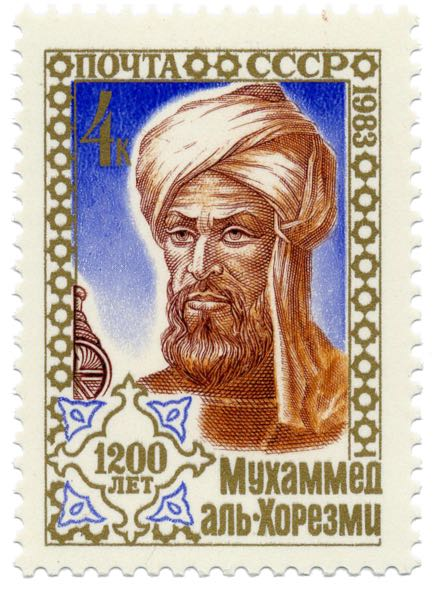
\includegraphics[height=4cm]{img5/juarismi} \par \footnotesize Al Juarismi (segle IX d.C) \par Pare de l'àlgebra.}{chap:algebra}
 
\vspace*{\fill} 
 
\begin{iniaval}  
\textbf{Classifica en vertaderes o falses les següents expressions:}

\begin{center}
	
\def\arraystretch{4}
\begin{longtable}{|p{1.1in}|p{1.1in}|p{1.1in}|p{1.1in}|} \hline 
\cellcolor{red!50}$\boldsymbol{a}\boldsymbol{+}\boldsymbol{a}\boldsymbol{\ =\ }\boldsymbol{2}\boldsymbol{\ }{\boldsymbol{a}}^{\boldsymbol{2}}$  & 
\cellcolor{green!50}$\boldsymbol{a}\boldsymbol{+}\boldsymbol{a}\boldsymbol{\ =\ }\boldsymbol{2}\boldsymbol{\ }\boldsymbol{a}$  & \textbf{2}$\boldsymbol{a}\boldsymbol{\textrm{·}}\boldsymbol{a}\boldsymbol{\ =\ }\boldsymbol{2}\boldsymbol{\ }{\boldsymbol{a}}^{\boldsymbol{2}}$  & $\boldsymbol{3}\boldsymbol{a}\boldsymbol{\textrm{·}}\boldsymbol{4}\boldsymbol{b}\boldsymbol{\ =\ }\boldsymbol{7}\boldsymbol{\ }\boldsymbol{ab}$  \\ \hline 
$\boldsymbol{a}\boldsymbol{\textrm{·}}\boldsymbol{b}\boldsymbol{\ =\ }\boldsymbol{ab}$  & $\boldsymbol{3}\boldsymbol{b}\boldsymbol{-}\boldsymbol{2}\boldsymbol{=}\boldsymbol{b}$  & $\boldsymbol{a}\boldsymbol{+}\boldsymbol{b}\boldsymbol{=}\boldsymbol{ab}$  & $\boldsymbol{a}\boldsymbol{:}\boldsymbol{2}\boldsymbol{=}\frac{\boldsymbol{a}}{\boldsymbol{2}}$  \\ \hline 
$\boldsymbol{b}\boldsymbol{\textrm{·}}\boldsymbol{3}\boldsymbol{\textrm{·}}\boldsymbol{a}\boldsymbol{\ =\ }\boldsymbol{3}\boldsymbol{\ }\boldsymbol{ab}$  & $\boldsymbol{3}\boldsymbol{a}\boldsymbol{\textrm{·}}\boldsymbol{4}\boldsymbol{b}\boldsymbol{\ =\ }\boldsymbol{12}\boldsymbol{\ }\boldsymbol{ab}$  & $\boldsymbol{2}\boldsymbol{a}\boldsymbol{+}\boldsymbol{b}\boldsymbol{\ =\ }\boldsymbol{2}\boldsymbol{\ }\boldsymbol{ab}$  & $\boldsymbol{2}\boldsymbol{\textrm{·}}\boldsymbol{a}\boldsymbol{\textrm{·}}\boldsymbol{a}\boldsymbol{\textrm{·}}\boldsymbol{b}\boldsymbol{=}\boldsymbol{2}{\boldsymbol{a}}^{\boldsymbol{2}}\boldsymbol{b}$  \\ \hline 
$\boldsymbol{3}\boldsymbol{b}\boldsymbol{-}\boldsymbol{3}\boldsymbol{b}\boldsymbol{=}\boldsymbol{b}$  & $\boldsymbol{3}\boldsymbol{\textrm{·}}\boldsymbol{a}\boldsymbol{\textrm{·}}\boldsymbol{a}\boldsymbol{\ =\ }\boldsymbol{6}\boldsymbol{\ }\boldsymbol{a}$  & $\boldsymbol{3}\boldsymbol{a}\boldsymbol{=}\boldsymbol{2}\boldsymbol{a}\boldsymbol{+}\boldsymbol{a}$  & $\boldsymbol{2}\boldsymbol{a}\boldsymbol{+}\boldsymbol{1}\boldsymbol{\ =\ }\boldsymbol{3}\boldsymbol{a}$  \\ \hline 
\end{longtable}

\end{center}


\addanswersline{Avaluació inicial}{0}{N'hi ha 8 de falses:\par $a+a=a^2$,\par $3a\cdot 4b=7ab$,\par $3b-2=b$,\par $a+b=ab$,\par $2a+b=2ab$,\par $3b-3b=b$,\par $3a\cdot a=6a$,\par $2a+1=3a$}

\end{iniaval}

\vspace*{\fill} 

\pagebreak

\section{El llenguatge algebraic}


\begin{theorybox}
	 \video[ytid=PJbIHC08-ho]{168}{El llenguatge algebraic} 
	 El llenguatge algebraic es caracteritza per utilitzar \textbf{números i lletres} (indeterminades). Normalment empram $x$, $y$, $\cdots$ per a les lletres.
	 
	 Si falta el signe de l'operació s'entén que hi ha una multiplicació. Primer s'escriu el número i després la lletra
	 \begin{center}
	 \be \quad \quad $\boxed{3\,x}$	\quad \quad\quad \quad \quad \quad  \malament  \quad \quad $\boxed{x\cdot3}$
	 \end{center}
 
	 Algunes expressions habituals són:
	 \begin{tasks}(2)
	 	\task[-] El doble d'un nombre: $2x$
	 	\task[-] Un nombre al quadrat: $x^2$
	 	\task[-] La meitat d'un nombre: $\frac{y}{2}$
	 	\task[-] L'anterior d'un nombre: $n-1$
	 	\task[-] Un nombre augmentat en 5 unitats: 
	 	
	 	$k+5$
	 	\task[-] El quadrat de la diferència de dos nombres: $(a-b)^2$
	 	\task[-] La diferència dels quadrats de dos nombres: $a^2 - b^2$
	 	\task[-] La mitjana de dues notes: $\frac{x+y}{2}$
	 \end{tasks}
	          
\end{theorybox}

\begin{mylist}



\exer  Escriu les expressions algebraiques que ens proporcionen l'àrea d'un quadrat i la longitud d'una circumferència.

\answers{l'àrea d'un quadrat = $x^2$ i la longitud d'una circumferència = $2\pi r$. Són monomis de grau 2 i 1 respectivament.}

\exer \spen  Escriu, en llenguatge algebraic, els següents enunciats, referits a dos nombres qualssevol \textit{x} i \textit{y}:
\begin{tasks}(1)
	\task  El triple de la seva diferència  \dotfill 
	\task  La suma dels seus quadrats   \dotfill
	\task  El quadrat de la seva suma  \dotfill
	\task  L'invers del seu producte  \dotfill 
	\task  La suma dels seus oposats  \dotfill 
	\task  El producte dels seus quadrats \dotfill
\end{tasks}

\answers{[$3(x-y)$, $x^2+y^2$, $(x+y)^2$, $\frac{1}{x\cdot y}$, $-x+(-y)$, $x^2\cdot y^2$]}

\exer  Suposem que tenim un contracte amb una companyia de telefonia mòbil pel qual paguem 5 cèntims d'euro per minut, així com 12 cèntims per establiment de cridada.  A la fi de cada mes l'empresa de telefonia mòbil ens proporciona la factura mensual. En ella apareix molta informació, en particular, el nombre total de cridades realitzades (\textit{N}) així com la quantitat total de minuts de conversa (\textit{M}). Troba una expressió que doni l'import de les cridades efectuades segons $N$ i $M$.

\redacta

\answers{L'import de la factura és $0,12 \cdot N + 0,05\cdot M$ euros.}


\exer  Una botiga de roba anuncia en els seus aparadors que està de rebaixes i que tots els seus articles estan rebaixats un 30~\% sobre el preu imprès en cada etiqueta. Escriu el que pagarem per una peça en funció del que apareix en la seva etiqueta. 

\answers{Pagarem el 70\% de $x=0.7 x$}

\exer  \spen Indica, en cada cas, el valor numèric de l'expressió $x-2y+3z$:  
\begin{tasks}(1)
	\task   $x=1,y=2,z=1$    \quad \examplebox{ \textbf{Exemple}: \quad    $x-2y+3z=1-2\cdot 2 + 3 \cdot 1=0$}
	\task   $x=2,y=0,z=-1$    
	\task   $x=0,y=1,z=0$    
\end{tasks}

\answers{[$0$, $-1$, $-2$]}

\exer  Calcula el valor numèric de les següents expressions algebraiques per al valor o els valors que s'indiquen:
\begin{tasks}(1)
	\task  \makebox[4cm]{ $\textit{x}{}^{2} + 2\textit{x} - 7$}   quan   $ x = 2$   
	\task \makebox[4cm]{  $\frac{a-3}{b+1}$}   quan    $a = -2$ i $\textit{b} = 4$   
	\task  \makebox[4cm]{$\textit{c}^{2} + 3\textit{c} + 7$ }   quan    $c = 1$
\end{tasks}

\answers{[$1$, $-1$, $11$]}

\exer  Calcula el valor numèric de les següents expressions algebraiques per al valor o valors que s'indiquen:
\begin{tasks}(1)
	\task  \makebox[5cm]{ $-3x^{2} +\frac{4}{x} -5$}  quan  $x=\frac{1}{2}$   
	\task \makebox[5cm]{  $3b+\frac{a+b}{2-b^{3} } +a\cdot b^{2} -1$ }  quan $a=3 $ i $b=1$
\end{tasks}

\answers{[$\frac{9}{4}$, $9$]}

\vspace{-3.75cm}
\exer \begin{minipage}[t]{0.75\textwidth}
	\simbolsearch Llança 2 daus. El resultat de cadascun serà el valor numèric de $x$ i $y$. Tot seguit, troba el valor numèric de les següents expressions amb els nombres que has obtingut: \vspace{0.25cm}
	
	\begin{tasks}(1)
		\task $x=\square$, \qquad $y=\square$ \qquad per a \quad  { $x+4y=$  }      \vspace{0.25cm}
		\task $x=\square$, \qquad $y=\square$ \qquad per a \quad  {  $(x+y)^2 - (x-y)^2=$ }   \vspace{0.25cm}
		\task $x=\square$, \qquad $y=\square$ \qquad per a \quad  {  $4x\cdot (1-y)=$ }    \vspace{0.25cm}
		\task $x=\square$, \qquad $y=\square$ \qquad per a \quad  {  $-x-(x^2+y^2)=$ }   \vspace{0.25cm}
	\end{tasks}
\end{minipage}
\begin{minipage}{0.24\textwidth}
	\centering
	\vspace{4.5cm}
	
\includegraphics[width=0.5\textwidth]{img5/color-dice}
\end{minipage}
Ara suma tots els resultats obtinguts i compara'l amb el teu company. Guanya la suma més gran. Quin deu ésser el valor més gran possible d'aquesta suma? Demana si algú de la classe ha obtingut aquest valor.
\answers{L'expressió simplificada de la suma és $4(x+y)-x^2-y^2$ i presenta un màxim a $x=y=2$. El valor màxim d'aquesta suma és 8.}
 
\end{mylist}

\section{Monomis}

\begin{theorybox}

\video[ytid=COY431F1xds]{169}{Monomis. Definició i operacions}  

Un \textbf{monomi} està format per un únic terme:   $-5\ xy^2$                 

\textbf{Coeficient}: $-5$,   \textbf{Part literal}: $xy^2$,

\textbf{Grau }(és la suma d'exponents): 3

\vspace{0.75cm}

\end{theorybox}

\vspace{2cm}
\begin{mylist}


\exer \spen En cadascun dels següents monomis escriu el seu coeficient, la seva part literal i el seu grau:

\begin{center}
\renewcommand*{\arraystretch}{1.4}
\begin{longtable}{|p{1.2in}|p{1.1in}|p{1.0in}|p{1.0in}|} \hline 
\rowcolor{lightgray} Monomi & Coeficient & Part literal & Grau \\ \hline 
$-12x^{3} $ &  &  &  \\ \hline 
$a^{4} b^{3} c$ &  &  &  \\ \hline 
$4xy^{2} $ &  &  &  \\ \hline 
\end{longtable}
\end{center}

\answers{ \begin{tabular}{|c|c|c|c|} \hline 
			\rowcolor{lightgray} Monomi & Coef & P.literal & Grau \\ \hline 
			$-12x^{3} $ & -12 & $x^3$ & 3 \\ \hline 
			$a^{4} b^{3} c$ & 1 & $a^{4} b^{3} c$ &  8  \\ \hline 
			$4xy^{2} $ & 4 & $xy^2$ & 3 \\ \hline 
		\end{tabular}
}

 \end{mylist}    

 

\subsection{Operacions amb monomis}

\begin{theorybox}


 \textbf{- Suma o resta de monomis:}           Només poden sumar o restar monomis amb la mateixa part literal. Sumam o restam els coeficients i copiam la part literal.

\begin{center}
	$\ 2x^2+5x^2-x^2=6x^2$    \quad\quad en canvi,\quad\quad    $2x^2+5x-y$  no es pot efectuar.
\end{center}
\vspace{0.25cm}

\textbf{- Producte de monomis: ``}\textit{Multiplicam coeficient amb coeficient i lletres amb lletres.''} 
\[2x^2\textrm{·}5x^3=2\textrm{·}5\ x^2\textrm{·}x^3=\ 10\ x^5\] 


\textbf{- Quocient de monomis: ``}\textit{Dividim coeficient amb coeficient i lletres amb lletres.''} 
\[4x^8:5x^5=\frac{4\ x^8}{5\ x^5}=\frac{4}{5}x^3\] 
\end{theorybox}

\begin{mylist}

\exer \spen Suma i resta els monomis equivalents.
\begin{tasks}(2)
\task $3x+5x =$ \examplebox{$8x$}
\task $11y+21y-7y =$ \examplebox{$25y$}
\task $5ab-18ab+7ab=$ \examplebox{$-6ab$}
\task $3x^5+7x^5=$
\task $4z^2+\frac{1}{2}z^2=$
\task $-x^2+\frac{1}{4}x^2=$
\task $x^4y^3+ \frac{1}{2}x^4y^3+\frac{1}{3}x^4y^3=$
\task $a-4a-(-8a+3a)+3a=$
\end{tasks}

\answers[cols=2]{[$8x$, $25y$, $-6ab$, $10x^5$, $\frac{9}{2}z^2$, $-\frac{3}{4}x^2$, $\frac{11}{6}x^4y^3$, $5a$]}

\exer \spen Fes el producte de monomis.
\begin{tasks}(2)
	\task $2x\cdot x \cdot x^2=$ \examplebox{$2x^4$}
	\task $4x^5\cdot 2x^7 =$ \examplebox{$8x^{12}$}
	\task $ \frac{1}{3}y^4 \cdot \frac{2}{5}y^2 =$
	\task $(-8x^2)\cdot \frac{1}{8}=$
	\task $(-\frac{3}{2}x^7)\cdot(-\frac{1}{3}x^4)\cdot (-x)=$
	\task $3x \cdot xy=$
	\task $5xy \cdot 3y^3 \cdot x^2y^2=$
	\task $a^2b^2 \cdot ab=$
\end{tasks}

\answers[cols=2]{[$2x^4$, $8x^{12}$, $\frac{2}{15}y^6$, $-x^2$, $-\frac{1}{2}x^{12}$, $6x^2 y$, $15x^3 y^6$, $a^3 b^3$]}

\newpage
\exer \spen Fes el quocient de monomis
 \begin{tasks}(2)
	\task $x^2:x=$\examplebox{$x$}
\task $x^3:2x^2=$\examplebox{$\frac{x}{2}$}
\task $3x^5:x^2=$
\task $\frac{8x^7}{2x^5}=$
\task $x^3:(2x^3)=$
\task $(-3)x^8:(-2x^3)=$
\task $\frac{-12x^3}{4x}=$
\task $3x^7:(-x^4)=$
\task $-9a:(3a)=$
\task $-10x^3y^2:(x^2y)=$
\task $3x^7:(-x^4)=$
\task $-5a^4b^3:(2a^3b)=$
\end{tasks}

\answers[cols=2]{[$x$, $\frac{x}{2}$, $3x^3$, $4x^2$, $\frac{1}{2}$, $\frac{3}{2}x^5$, $-3x^2$, $-3x^3$, $-3$, $-10xy$, $-3x^3$, $-\frac{5}{2}a b^2$]}

\exer \spen Fes les operacions combinades. 
 \begin{tasks}(2)
	\task $(4x^2:2x)\cdot x=$\examplebox{$2x^2$}
	
\task $(-2x\cdot 5x^2):(2x)=$\examplebox{$-5x^2$}

\task $xy\cdot (x+3x)=$

\task $(12 x^3y^3 -7x^3y^3): (3x^2y)=$

\task $2\frac{x^5}{x^3}+ 2 \frac{x^4}{x^2} + 2 \frac{x^2}{x^0}=$

\task $(ab^2)\cdot a + (a^2 b)\cdot (3b)=$

\task $(ab):a - (7b^2+b^2):b=$

\task $\frac{\frac{x^2y^2}{xy}+\frac{3}{2}xy+\frac{7x^4y}{3x^3}}{\frac{3}{2}y}=$
 \end{tasks}

\answers[cols=2]{[$2x^2$, $-5x^2$, $4x^2 y$, $\frac{5}{3} x y^2$, $6x ^2$, $4 a^2 b^2$, $-7b$, $\frac{29}{9}x$]}

\end{mylist}


\section{Operacions amb polinomis}

\begin{theorybox}
\begin{multicols}{2}
	\centering
 \videonw[ytid=dOSn5n9k09]{170}{Polinomis: Definició. Suma i resta.}
 \videonw[ytid=3M7-s6U2oXw]{171}{Producte de polinomis}                     
 \end{multicols}

 Un \textbf{polinomi} està format per la suma o resta de \textbf{molts} de \textbf{monomis}. 
 
 Per exemple $9x^2-2x+5$, està format per 3 termes. Té grau 2 que és el major grau dels seus monomis. El seu terme independent és 5 (correspon al terme de grau 0) .
\end{theorybox}

\newpage
\begin{mylist}
	
	
\exer \spen Completa la taula

\begin{center}
	\renewcommand*{\arraystretch}{1.6}
	\begin{longtable}{|p{1.2in}|p{1.1in}|p{1.0in}|p{1.0in}|} \hline 
		\rowcolor{lightgray} Polinomi & N. Termes & Grau & Terme \par independent \\ \hline 
		$5x^{4} +7x^{2}$ &  &  &  \\ \hline 
		$6x^{2} +10-2x^{3} $ &  &  &  \\ \hline 
		$3x^{4}-5x^{3}+x^2+1 $ &  &  &  \\ \hline 
		$2xy^{3} -x^{5} +7x^{2} y^{2}$ &  &  &  \\ \hline 
	\end{longtable}
\end{center}
 
 \answers{ 	\begin{tabular}{|c|c|c|c|} \hline 
 			\rowcolor{lightgray} Poli. & Termes & Grau & T.I. \\ \hline 
 			$5x^{4} +7x^{2}$ & 2 & 4 & 0 \\ \hline 
 			$6x^{2} +10-2x^{3} $ & 3  & 3 &  10 \\ \hline 
 			$3x^{4}-5x^{3}+x^2+1 $ & 4 & 4 & 1 \\ \hline 
 			$2xy^{3} -x^{5} +7x^{2} y^{2}$ & 4 & 5 & 0 \\ \hline 
 		\end{tabular}}

\exer \spen Sigui el polinomi $P(x)=x^{3} -3x+2$. Troba els següents valors numèrics de $P(x)$:


 $P(0)=$
  
  $P(1)=$
  
   $P(-1)=$
   
   $P(-2)=$ 
   
   
    $P(1/2)=$   


\answers{[$2$, $0$, $4$, $0$, $\frac{5}{8}$]}


\exer \spen  Realitza les següents sumes de polinomis:

\begin{tasks}(1)
	\task  $(-x^{3} +x-5)+(2x^{2} +5x+4)+(-4x^{3} -2x^{2} +3x)=$
	
	\task   $(x^{2} +4)+(-2x+4)+(-6x^{3} +3x^{2} +x+1)-x^{2}= $
\end{tasks}

\answers{[$-5x^3+9x-1$, $-6x^3+3x^2-x+9$]}


\exer  \spen Realitza les següents diferències. (Canvia tots els signes del subtrahend) 
\begin{tasks}(1)
\task   $(5x^{2} +2)-(-2x)=$

\task   $(-2x^{3} +4x)-(-2x-1)=$            

\task  $ (7x^{2} -2x)-(3x^{3} +4x^{2} -x+1)=$
\end{tasks}

\answers{[$5x^2+2x+2$, $-2x^3+6x+1$, $-3x^3+3x^2-x-1$]}

\begin{comment}

\exer  Escriu el polinomi oposat (canviat de signe) de cadascun dels següents polinomis: 
\begin{tasks}(3)
    \task $2x^{3} -2x^{2} -3x+9$   
	\task  $-5x$   
	\task  $-x^{3} +7x$ 
\end{tasks}


\exer  Obté el valor del polinomi $P(x)= 4x^{3} -x^{2} +1$ en $x=2$. Quin valor pren el polinomi oposat de  $P$ en $x=2$? 

\end{comment}

\exer  Considera els polinomis $P(x)= x^{2} -x+1$, $Q(x)= -x^{3} +2x-3$, així com el polinomi suma $S=P+Q$. Troba els valors de cadascun d'ells per a $x=-2$, és a dir, calcula $P(-2)$, $Q(-2)$ i $S(-2)$. Investiga si existeix alguna relació entre aquests tres valors.   

\answers{El polinomi suma $S(x)=-x^3+x^2+x-2$; els valors numèrics $P(-2)=7$, $Q(-2)=1$ i $S(-2)=8$. Es compleix que $S(-2)=P(-2)+Q(-2)$. }

\exer  Fes aquestes multiplicacions de monomi per polinomi:
\begin{tasks}(2)
	\task $x\cdot (x^2+3x-1)=$
	\task $3x\cdot (-2x+5)=$
	\task $-2x^2\cdot (3x^5 - 4x^2 + 8x)=$
	\task $\frac{3}{2}x^3\cdot (6x^4 + 2)=$
\end{tasks}  

\answers{[$x^3+3x^2-x$, $-6x^2+15x$, $-6x^7+8x^4-16x^3$, $9x^7+3x^3$]}

\exer \spen De cadascun dels següents polinomis extreu els factors que siguin comuns als seus monomis:

\begin{tasks}(2)
	\task  $2x^2+2x+2=$ \examplebox{$2\cdot (x^2+x+1)$}
	   
	\task  $x^2+x=$ \examplebox{$x\cdot (x+1)$} 
	
	\task  $15x^2+5x=$
	   
	\task  $-16x^2-4x-8=$   
	   
	\task  $-10x^{3} -15x^{2} +20x=$   
	
	\task  $30x^{4} +24x^{2}=$
\end{tasks}

\answers{[$2(x^2+x+1)$, $x(x+1)$, $5x(3x+1)$, $-4(4x^2+x+2)$, $-5x(2x^2+3x-4)$, $6x^2(5x^2+6)$]}

\exer  Efectua els següents productes de polinomis:
\begin{tasks}(2)
	\task $(-2x)\cdot (3x^{2} -4)=$
	\task $(2x^{3} +1)\cdot (-4x+5)=$
	\task $(4x^{3} -x^{2} -1)\cdot (2x+6)=$
	\task $(-1)\cdot (8x^{2} +7x-9)=$
\end{tasks}  

 \answers{[$-6x^3+8x$, $-8x^4+10x^3-4x+5$, $8x^4+22x^3-6x^2-2x-6$, $-8x^2-7x+9$]}

\exer  Calcula i simplifica els següents productes: 

\begin{tasks}(2)
	\task   $x\cdot (-2x+4)$     
	\task   $(2x-3)\cdot (3x+2)$    
	\task   $(a-2)\cdot (4-3a)$  
	\task   $(3a-b^{2} )\cdot (2b-a^{2} )$ 
\end{tasks}

\answers{[$-2x^2+4x$, $6x^2-5x-6$, $-3a^2+10a-8$, $-3a^3 + a^2b^2+6ab-2b^3$]}


\exer[1]  Realitza els següents productes de polinomis:

\begin{tasks}(2)
	\task  $x\cdot (-3x^{2} +4x+2)\cdot x^{2} $  
	\task $(-2x+1)\cdot (5x^{2} -x+3)\cdot (-x)$  
	\task  $(3a-1)\cdot (2-a)\cdot (5-4a)$
\end{tasks}
\answers[cols=1]{[$-3x^5+4x^4+2x^3$, $10x^4-8x^3+7x^2-3x$, $12\,a^3-43\,a^2+43\,a-10$]}

\end{mylist}

\subsection{Divisió de polinomis}

\begin{theorybox}
En una divisió de dos polinomis
\[ 
	\begin{array}{lll}
	D(x) & & |\underline{d(x)\quad} \\
	\underbrace{R(x)} & & Q(x)
	\end{array}
\]

$D(x)$ s'anomena dividend, $d(x)$ divisor, $Q(x)$ quocient i $R(x)$ el residu. En el cas que el residu sigui zero, es diu que la \textbf{divisió és exacta}.

La comprovació que una divisió està ben feta és:
\[ \boxed{ D(x)= Q(x)\cdot d(x) + R(x)}  \]

Si el divisor és de la forma $x-a$ o $x+a$, aleshores podem utilitzar la \textbf{regla de Ruffini}. Recorda que quan falta algun terme en el dividend cal afegir zeros quan feim Ruffini.
   

   
\end{theorybox}

\pagebreak

\begin{example}
 	$\bullet$ Comprova que els càlculs que tens a continuació reflecteixen la divisió del polinomi
	
	 $p(x)=6x^{4} +5x^{3} +x^{2} +3x-2$ entre el polinomi $q(x)=2x^{2} -x+3$:
	
	
	\[ \begin{array}{l} {\, \, \, \, 6x^{4} +5x^{3} +x^{2} +3x-2\quad \quad \quad \quad \underline{|}\underline{\quad 2x^{2} -x+3}\underline{\quad }} \\ {\underline{-6x^{4} +3x^{3} -9x^{2} }\, \, \, \, \, \, \, \, \, \, \, \, \, \, \, \, \, \, \, \, \, \, \, \, \, \, \, \, \, \, \, \, \, \, \, \, \, \, \, \, \quad 3x^{2} +4x-2\, } \\ {\, \, \, \, \, \, \, \, \, \, \, \, \, \, \, \, 8x^{3} -8x^{2} +3x-2} \\ {\, \, \, \, \, \, \, \, \, \, \, \, \underline{-8x^{3} +4x^{2} -12x}} \\ {\, \, \, \, \, \, \, \, \, \, \, \, \, \, \, \, \, \, \, \, \, \, \, \, -4x^{2} -9x-2} \\ {\, \, \, \, \, \, \, \, \, \, \, \, \, \, \, \, \, \, \, \, \, \, \, \, \, \, \, \, \underline{4x^{2} -2x+6}} \\ {\, \, \, \, \, \, \, \, \, \, \, \, \, \, \, \, \, \, \, \, \, \, \, \, \, \, \, \, \, \, \, \, \, \, \, \underbrace{-11x+4} } \end{array} \]
	
	
	$\bullet$ Realitza aquesta divisió $(x^3+5x-2) : (x-4)$ per la regla de Ruffini:
	
	\[ \begin{array}{r|rrrr}  & 1 & 0 & 5 & -2\\ 4 &  & 4 & 16 & 84 \\ \hline  & 1 & 4 & 21 & \examplebox{ 82 }\end{array} \]
	
	El quocient és $Q(x)=x^2+4x+21$ i el residu de la divisió $R=82$.
	\end{example}

\begin{mylist}

\exer[1]  Divideix els següents polinomis:   
\begin{tasks} 
   \task \makebox[6cm]{$3x^{3} +4x^{2} -9x+7$} entre \quad $x^{2} +2x-1$
   \task \makebox[6cm]{$-6x^{3} +2x^{2} +3x+4$} entre \quad $3x^{3} +x^{2} -2x+1$
   \task \makebox[6cm]{$-6x^{4} -13x^{3} -4x^{2} -13x+7$} entre\quad $-3x^{2} -2x+1$ 
   \task \makebox[6cm]{$3x^{5} -9x^{4} +7x^{3} +4x^{2} -14x+14$} entre \quad $x^{3} -2x^{2} -x+3$ 
   \task \makebox[6cm]{$x^{5} -4x-6$} entre \quad $x^{2} +3$ 
\end{tasks}
\answers[cols=1]{[$Q=3x-2$; $R=-2x+5$, $Q=-2$; $R=4x^2-x+6$, $Q=2x^2+3x$; $R=-16x+7$, $Q=3x^2-3x+4$; $R=-x+2$, $Q=x^3-3x$; $R=5x-6$]}

\exer[1]  Efectua les següents operacions utilitzant \textbf{la regla de Ruffini} i indica quines d'elles són exactes.
\begin{tasks} 
  \task  $\left(3x^2-\ 2x\ +\ 5\right):\left(x+3\right)$
  \task  $\left(x^4-\ 16\right):\left(x-2\right)$
  \task  $\left(x^4-x^3+x^2-x+1\right):\left(x-1\right)$
   \task $\left(7x^5-\ 4x^3+7x-\ 5\right):\left(x+2\right)$
\end{tasks}
\answers[cols=1]{[$Q=3x-11$; $R=38$, $Q=x^3+2x^2+4x+8$; $R=0$, $Q=x^3+x$; $R=1$, $Q=7x^4-14x^3+24x^2-48x+103$; $R=-211$]}


 


\exer  Efectua les divisions de polinomis pel mètode que creguis més convenient: 

\begin{tasks} 
	\task  \makebox[6cm]{$2x^{3} +x^{2} -12x+7$} entre \quad $x+3$    
	\task  \makebox[6cm]{$-4x^{4} +8x^{3} +7x^{2} -21x+8$} entre \quad $2x^{2} -3x+1$
	\task  \makebox[6cm]{$-3x^{5} -2x^{3} +9x^{2} +6x-14$} entre \quad $-x^{3} -2x+3$
\end{tasks}

\answers[cols=1]{[$Q=2x^2-5x+3$; $R=-2$, $Q=-4x^4+8x^3+7x^2-21x+8$; $R=2x^2-3x+1$, $Q=3x^2-4$; $R=-2x-2$]}

\exer  Troba dos polinomis tals que en dividir-los obtinguem $q(x)=x^{2} -2x-1$ com a polinomi quocient i $r(x)=2x^{2} -3$ com a residu. 

\answers{Hi ha infinites solucions. Per exemple, si ens inventam el divisor=$2x+3$, el dividend=quocient·divisor + residu = $(x^2-2x-1)(2x+3)+2x^2-3=2x^3+x^2-8x-6$} 

\end{mylist}


\section{Identitats notables}


\begin{theorybox}
	
	\video[ytid=xfVp1cXpKb4]{172}{Identitats notables}
	
	\makebox[4cm][l]{Quadrat d'una suma:}   ${\left(\boldsymbol{a}\boldsymbol{+}\boldsymbol{b}\right)}^{\boldsymbol{2}}\boldsymbol{=\ }{\boldsymbol{a}}^{\boldsymbol{2}}\boldsymbol{+}\boldsymbol{2}\boldsymbol{\textrm{·}}\boldsymbol{a}\boldsymbol{\textrm{·}}\boldsymbol{b}\boldsymbol{+}{\boldsymbol{b}}^{\boldsymbol{2}}$ 
	
	\makebox[4cm][l]{Quadrat d'una diferència:}   ${\left(\boldsymbol{a}\boldsymbol{-}\boldsymbol{b}\right)}^{\boldsymbol{2}}\boldsymbol{=\ }{\boldsymbol{a}}^{\boldsymbol{2}}\boldsymbol{-}\boldsymbol{2}\boldsymbol{\textrm{·}}\boldsymbol{a}\boldsymbol{\textrm{·}}\boldsymbol{b}\boldsymbol{+}{\boldsymbol{b}}^{\boldsymbol{2}}$       
	
	\makebox[4cm][l]{Suma per diferència:} $\left(\boldsymbol{a}\boldsymbol{+}\boldsymbol{b}\right)\boldsymbol{\textrm{·}}\left(\boldsymbol{a}\boldsymbol{-}\boldsymbol{b}\right)\boldsymbol{=\ }{\boldsymbol{a}}^{\boldsymbol{2}}\boldsymbol{-}{\boldsymbol{b}}^{\boldsymbol{2}}$
	\vspace{0.5cm}
\end{theorybox}

\begin{mylist}

\exer \spen  Desenvolupa les identitats:

\begin{tasks}(2)
	\task  $(1+x)^{2}= $    
	
	\task  $(-x+2)^{2}= $     
	
	\task  $(x-2)^{2} =$ 
	
	\task  $(2a-3)^{2}= $      
	
	\task $\left(x^{2} +1\right)^{3}= $      
	
	\task $(2b-4)^{3}= $
\end{tasks}

\answers[cols=2]{[$1+2x+x^2$, $x^2-4x+4$, $x^2-4x+4$, $4a^2-12a+9$, Atenció 3: $x^6+3x^4+3x^2+1$, Atenció 3: $8b^3-48b^2+96b-64$]}


\exer \spen  Efectua aquests productes:

\begin{tasks}(2)
	\task  $(3x+2)\cdot (3x-2)=$    

	\task  $(2x+4y)\cdot (2x-4y)=$   

	\task  $(4x^{2} +3)\cdot (4x^{2} -3)=$

	\task  $(3a-5b)\cdot (3a+5b)=$   
	
	\task  $(x^{3} -4)\cdot (x^{3} +4)=$ 

	\task  $\left(-x^{2} +5x\right)\cdot \left(x^{2} +5x \right)=$ 
\end{tasks}

\answers{[$9x^2-4$, $4x^2-16y^2$, $16x^4-9$, $9a^2-25b^2$, $x^6-16$, $-x^4+25x^2$]}

\exer \spen  Desenvolupa les següents potències: 

\begin{tasks}(2)
	\task  $(3x-y)^2=$
	
	\task  ${\left(2a\ +\ \frac{x}{2}\right)}^2=$   
	
	\task  ${\left(4y-\ \frac{2}{y}\right)}^2=$ 
	
	\task  $\left(5a+a^2\right)^2=$
	 
	\task  $\left( -a^2+2b^2 \right)^2=$ 
	 
	\task  ${\left(\frac{2}{3}y-\ \frac{1}{y}\right)}^2=$ 
\end{tasks}

\answers{[$9x^2-6xy+y^2$, $4a^2+2ax+\frac{x^2}{4}$, $16y^2-16+\frac{4}{y^2}$, $25a^2+10a^3+a^4$, $a^4-4a^2b^2+4b^4$, $\frac{4y^2}{9}-\frac{4}{3}+\frac{1}{y^2}$]}

\pagebreak
\exer \spen Expressa com quadrat d'una suma o d'una diferència les següents expressions algebraiques:

\begin{tasks}(2)
	\task  ${a}^{2} - 6{a +} 9 = \left(\square - \square \right)^2$   
	\task  $4{x}^{2} + 4x + 1 =$   
	\task  ${b}^{2} - 10{b} + 25=$
	\task  $4{y}^{2} - 12{y} + 9 =$   
	\task  ${a}^{4} + 2{a}^{2} +1=$    
	\task  ${y}^{4} + 6x{y}^{2} + 9{x}^{2}=$
\end{tasks}

\answers{[$(a-3)^2$, $(2x+1)^2$, $(b-5)^2$, $(2y-3)^2$, $(a^2+1)^2$, $(y^2+3x)^2$]}

\vspace{0.5cm}

\exer \spen  Expressa com suma per diferència les següents expressions

\begin{tasks}(2)
	\task  $9x^2-25 = \left(\square + \triangle \right) \cdot \left(\square - \triangle \right)  $    
	\task  $4 a^4 - 81 b^2 =$   
	\task  $49-25x^2 =$ 
	\task  $100 a^2 -64=$
\end{tasks}

 \answers{[$(3x+5)(3x-5)$, $(2a^2+9b)(2a^2-9b)$, $(7+5x)(7-5x)$, $(10a+8)(10a-8)$]} 
\vspace{0.5cm}

\exer  Realitza les següents divisions de polinomis a partir de la conversió del dividend en la potència d'un binomi o en un producte de la forma suma per diferència:

\begin{tasks}(2)
	\task $x^{2} +12x+36$    entre $x+6$      
	\task  $4x^{4} -16x^{2} $ entre $2x^{2} -4x$ 
	\task  $9x^{2} -24x+16$ entre $3x-4$     
	\task  $x^{2} -4$  entre $x+2$   
\end{tasks}

\answers[cols=1]{[$(x+6)^2 / (x+6)=x+6$, $(2x^2+4x)(2x^2-4x)/(2x^2-4x)=2x^2+4x$, $(3x-4)^2/(3x-4)=3x-4$, $(x+2)(x-2)/(x+2)=x-2$]}
\vspace{0.5cm}


\exer \hot  Obté les fórmules dels quadrats dels següents trinomis:

\begin{tasks}(2)
	\task $(a+b+c)^{2} $    
	\task  $(a-b+c)^{2} $ 
\end{tasks}

\answers{[$a^2+b^2+c^2+2ab+2ac+2bc$, $a^2+b^2+c^2-2ab+2ac-2bc$]}


\end{mylist}


\section{Introducció a les fraccions algebraiques}

\begin{theorybox}

 Una fracció algebraica és el quocient de dos polinomis $\frac{D\left(x\right)}{d\left(x\right)}$

 Si la divisió $D(x):d(x)$ és exacta, la fracció serà en realitat un polinomi.

 Per \textbf{sumar/restar fraccions} necessitam denominador comú:
\[\frac{2x}{x-1}+\frac{3}{x+2}=\frac{2x\textrm{·}(x+2)}{(x-1)(x+2)}+\frac{3(x-1)}{(x-1)(x+2)}=\frac{2x\textrm{·}\left(x+2\right)+3\left(x-1\right)}{(x-1)(x+2)}=\frac{2x^2+7x-3}{x^2+x-2}\] 
Per \textbf{multiplicar fraccions}, multiplicam ``en línia´´:
\[\frac{2x}{x-1}\textrm{·}\frac{3(x+2)}{x+1}=\frac{2x\textrm{·}3(x+2)}{(x-1)(x+1)}=\frac{6x^2+12x}{x^2-1}\] 
Per \textbf{dividir fraccions}, multiplicam ``en creu´´:
\[\frac{2x}{x-1}:\frac{3(x+2)}{x+1}=\frac{2x\textrm{·}(x+1)}{3(x-1)(x+2)}=\frac{2x^2+2x}{3x^2+3x-6}\] 
\end{theorybox}

\begin{mylist}

\exer[1]  Efectua els següents càlculs: 

\begin{tasks}(2)
	\task  $\frac{1}{x+2} +\frac{2}{x-1} $   
	\task $\frac{x-2}{x^{2} -x} -\frac{5}{x} $   
	\task $\frac{-x+1}{x+3} \cdot \frac{3x^{2} }{x+1} $   
	\task $\frac{2+x}{x^{2} } :\frac{x}{x-3} $
\end{tasks}
\answers{[$\frac{3x+3}{x^2+x-2}$, $\frac{-4x+3}{x^2-x}$, $\frac{-3x^3+3x^2}{x^2+4x+3}$, $\frac{x^2-x-6}{x^3}$]}

\exer[1]  Realitza les següents operacions alterant, en cada apartat, solament un dels denominadors, i el seu respectiu numerador: 

\begin{tasks}(2)
	\task $\frac{-2x^{2} -x+1}{x^{3} } +\frac{3x+1}{x^{2} } $    
	\task $\frac{2x-1}{x^{2} -2x} -\frac{3}{x-2} $
\end{tasks}
\answers{[$\frac{x^2+1}{x^3}$, $\frac{-x-1}{x^2-2x}$]}

\exer  Calcula els següents quocients (treu factor comú del numerador):  

\begin{tasks}(2)
	\task  (2\textit{x}${}^{3}$ $-$ 8\textit{x}${}^{2}$ + 6\textit{x}) : 2\textit{x    }
	\task  (5\textit{a}${}^{ 3}$ + 60\textit{a${}^{ 2}$} $-$ 20) : 5  
	\task  (16\textit{x}${}^{3}$ + 40\textit{x}${}^{2}$) : 8${x}^{2 }$   
	\task  (6\textit{x}${}^{2}$y${}^{3}$ $-$ 4\textit{xy${}^{2}$}) : \textit{xy}${}^{2}$
\end{tasks}
\answers{[$x^2-4x+3$, $a^3+12a^2-4$, $2x+5$, $6xy-4$]}


\end{mylist}
 
\begin{resolt}{Simplifica la fracció algebraica \[ \frac{x^2-2x}{x^2 - 4} \]}
	La primera passa consisteix en factoritzar el numerador i el denominador. Per això ens fixam si podem treure factor comú i/o identificam alguna identitat notable.
	
	\[ \frac{x^2-2x}{x^2 - 4} = \frac{x \cdot \cancel{(x-2)}}{(x + 2)\cdot \cancel{(x-2)}} = \frac{x}{x + 2} \]
	
	Finalment, hem eliminat els factors que estan repetits al numerador i denominador.
\end{resolt}
 
\begin{mylist}

\exer  Comprova les següents identitats simplificant l'expressió del costat esquerre de cada igualtat: 

\begin{tasks}(2)
	\task $\frac{6a^{8} b^{2} }{2a^{3} b} =3a^{5} b$    
	\task  $\frac{8x^{3} y-2xy^{2} }{4xy} =2x^{2} -\frac{1}{2} y$ 
	\task $\frac{4x^{2} +2x}{2x-8} =\frac{2x^{2} +x}{x-4} \quad $   
	\task  $\frac{6a^{2} b^{2} -4a^{2} b^{3} +4ab}{2ab^{2} -8a^{2} b} =\frac{3ab-2ab^{2} +2}{b-4a} $
\end{tasks}

\exer  Simplifica les següents fraccions traient factor comú:

\begin{tasks}(2)
	\task  $\frac{3x^{2} +6x}{9x^{2} +18} $   
	\task  $\frac{a^{3} -7a^{2} }{3a^{3} +5a^{2} } $   
	\task  $\frac{x^{2} y^{2} -7xy^{2} }{2xy} $   
	\task $\frac{a^{2} b^{2} -ab}{a^{3} b+ab} $
\end{tasks}


\answers[cols=1]{[$\frac{3x(x+2)}{3(3x^2+6)}=\frac{x(x+2)}{3x^2+6}$,
	$\frac{a^2(a-7)}{a^2(3a+5)}=\frac{a-7}{3a+5}$,
	$\frac{ay(xy-7y)}{2xy}=\frac{y(x-7)}{2}$,
	$\frac{ab(ab-1)}{ab(a^2+1)}=\frac{ab-1}{a^2-1}$]}


\exer[1] En cadascuna de les següents fraccions algebraiques escriu, quan sigui possible, el polinomi numerador, o denominador, en forma de potència d'un binomi o de suma per diferència per, posteriorment, poder simplificar cada expressió: 

\begin{tasks}(4)
	\task  $\frac{x^{2} -4}{3x+6} $    
	\task $\frac{2x^{2} -16x+32}{x^{2} -16} $   
	\task  $\frac{6-4a}{4a^{2} -9} $
	\task  $\frac{x^2+2x}{x^2-4}$
\end{tasks}
\answers[cols=2]{[$\frac{x-2}{3}$, $\frac{2(x-4)}{x+4}$, $\frac{-2}{2a+3}$, $\frac{x}{x-2}$]}
\end{mylist}




\pagebreak
\begin{activitats}
	
\begin{mylist}

\exer  Una empresa majorista de viatges està confeccionant una oferta per distribuir-la en diferents agències de viatges. Es tracta d'un viatge amb avió, d'anada i tornada, a Madrid el preu de la qual dependrà del nombre final de viatgers. Les dades concretes són: 

\begin{tasks}
	\task[-]  Si no hi ha més de 100 persones interessades, el vol costarà 150 euros per persona.
	\task[-]  Si hi ha més de 100 persones interessades, per cada viatger que passi del centenar el preu del viatge es reduirà en 1 euro. No obstant això, el preu del vol en cap cas serà inferior a 90 euros.
\end{tasks}
Estudia i determina el preu final del vol, per persona, en funció del nombre total de viatgers. Així mateix, expressa la quantitat que ingressarà l'empresa segons el nombre de viatgers. 

\answers{	Anomenarem $n$ al nombre de viatgers, $p$ al preu per viatger i $T$ a la quantitat total ingressada per l'empresa.\par
	Tots els valors de les variables són nombres enters.\par
	Si $n <101$: $P = 150$; $T = 150N$\par
	Si $n = 100 + x (0 <x <61)$: $p = 150 - x$; $T = 15 000 + 50x - x^2$\par
	Si $n> 160$: $p = 90$; $T = 90N.$}

\exer  En aquest exercici es mostra un \textit{truc} mitjançant el qual anem a endevinar el nombre que resulta després de manipular repetidament un nombre desconegut. Converteix en una expressió algebraica les successives alteracions del nombre desconegut i justifica el que ocorre.  
  
  \begin{itemize}
 \item Digues-li a un company que escrigui en un paper un nombre parell i que no ho mostri   

 \item Que ho multipliqui per 5

\item Que al resultat anterior li sumi 5 

\item  Que multipliqui per 2 el resultat

 \item Que al resultat anterior li sumi 10

 \item Que multipliqui per 5 

 \item  Que divideixi entre 100 la darrera quantitat 
 
 \item  Que al resultat precedent li resti la meitat del nombre que va escriure

\end{itemize} 

Independentment del nombre desconegut original quin nombre ha sorgit?

\answers{	Si anomenam $2n$ al nombre parell inicial, la seqüència d'operacions dóna lloc a $\frac{[(10n+5)\cdot 2 -10]\cdot 5}{100}-n = 0$. 
}

\exer  Els responsables d'una empresa, en previsió d'uns futurs alts i baixos en les vendes dels productes que fabriquen, pensen proposar als seus treballadors a la fi de l'any 2014 el següent: 
\begin{itemize}
\item  La disminució dels sous, per al proper any 2015, en un 10\%. 

\item  Per 2016 ofereixen augmentar un 10\% els salaris de 2015.

\item  En general, suggereixen que el sou disminueixi un 10\% cada any imparell i que augmenti un 10\% cada any parell. 
\end{itemize}

 Si finalment s'aplica aquest pla, estudia si els treballadors recuperaran l'any 2016 el salari que tenien en 2014. Analitza què ocorre amb els sous després del pas de molts anys.

\answers{  Si anomenem $s$ al salari de 2014, els salaris dels anys successius són:\par
	$0,9 s$; $0,99 s$; $0,891 s$; $0,9801 s$; $0,88209 s$; $0,970299 s$; ...
	Els salaris són cada vegada menors que dos anys abans.}


\begin{comment}
\exer  Els responsables de l'anterior empresa, després de rebre l'informe d'una consultora, alteren la seva intenció inicial i van a proposar als seus treballadors, a la fi de l'any 2014, el següent: 


\exer 
\exer  Un augment dels sous, per al proper any 2015, d'un 10\%. 

\exer  Per 2016, una reducció del 10\% sobre els salaris de 2015.

\exer  En general, suggereixen que el sou augmenti un 10\% cada any imparell i que disminueixi un 10\% cada any parell. 




 Si s'aplica el nou pla, analitza si el salari dels treballadors de l'any 2016 coincidirà amb el que tenien en 2014. Estudia com evolucionen els sous després del pas de molts d'anys.

\end{comment}



\exer  Observa si hi ha nombres pels quals les següents expressions no poden ser avaluades:

\begin{minipage}{0.22\textwidth}
	\begin{tasks}
		\task  $\frac{x-3}{x+1} $  
		\task $\frac{2x-1}{(x-5)\cdot (2x+7)} $   
		\task $\frac{x}{x^{2} -2x+1} $   
		\task $\frac{x+y-2}{x^{2} +3y^{2} } $
	\end{tasks}
\end{minipage}
\begin{minipage}{0.2\textwidth}
	\centering
	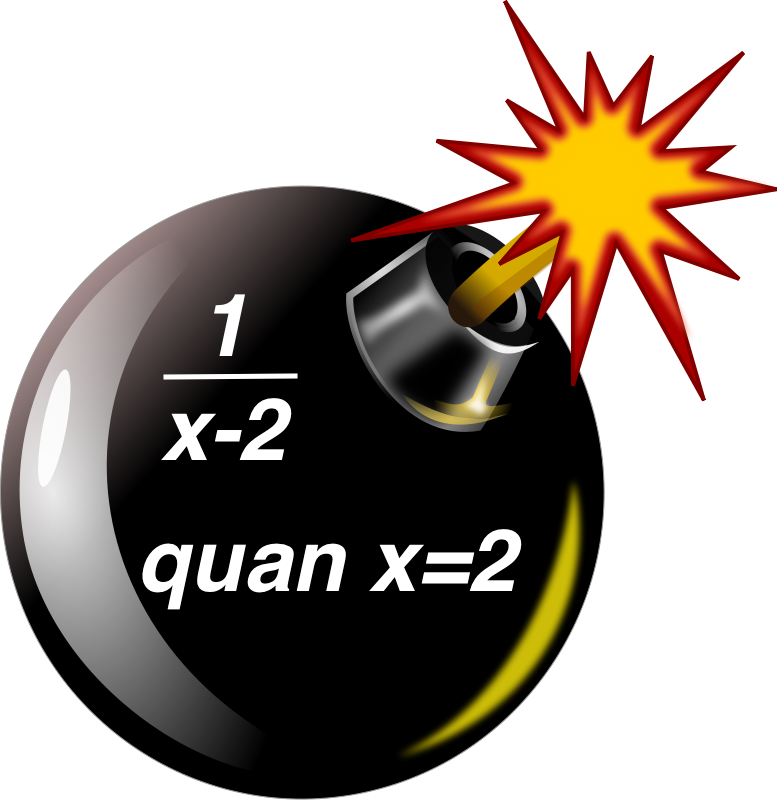
\includegraphics[width=0.85\textwidth]{img5/bomb}
\end{minipage}

\answers{[Per a $x=-1$, Per a $x=5$ ni $x=-7/2$, Per a $x=1$, Es pot avaluar per tot $x$; $y$]}

\begin{comment}
\exer  Una persona té estalviats 3000~€ i decideix dipositar-los en un producte bancari amb un tipus d'interès anual del 2,5~\%. Si decideix recuperar els seus estalvis al cap de dos anys, quin serà la quantitat total de la qual disposarà?
\end{comment}

\exer  Construeix un polinomi de grau 2, $P(x)$, tal que $P(-2)=6$.

\answers{Per exemple: $(x+2)^2 + 6 = x^2 + 4x + 10$}

\exer  Considera els polinomis $p(x)=2x^{3} -x^{2} +4x-1$, $q(x)=-x^{4} -3x^{3} +2x^{2} -x-5$ i $r(x)=x^{2} -3x+2$ . Fes les següents operacions:  

\begin{tasks}(2)
	\task  $p+q+r$   
	\task $p-q$   
	\task $p\cdot r$   
	\task $p\cdot r-q$
\end{tasks}

\answers[cols=1]{ $p+q+r=-x^4-x^3+2\,x^2-4$, \par
	 $p-q=x^4+5\,x^3-3\,x^2+5\,x+4$,    \par
	 $p\cdot r=2\,x^5-7\,x^4+11\,x^3-15\,x^2+11\,x-2$,    \par
	 $p\cdot r-q=2\,x^5-6\,x^4+14\,x^3-17\,x^2+12\,x+3$}

\pagebreak
\exer  Calcula els productes:

\begin{tasks}
	\task  $\left(\frac{3ax}{2} -\frac{y}{5} \right)\cdot \left(\frac{-by}{3} \right)$  
	\task  $\left(0'1x+0'2y)\right)\cdot \left(0'3x-0'2y\right)$  
	\task  $\left(x-y\right)\cdot \left(y-1\right)\cdot \left(x+a\right)$
\end{tasks}

\answers{[$\frac{by^2}{15}-\frac{1}{2}abxy$, $0.03x^2 + 0.04 xy - 0.04 y^2$, $a x y - a x - a y^2 + a y + x^2 y - x^2 - x y^2 + x y$]}

\exer  Calcula els quocients: 
\begin{tasks}
	\task  $(4x^{3} ):(x^{2} )$ 
	\task  $\left(4x^{3} y^{3} z^{4} \right):\left(3x^{2} yz^{2} \right)$  
	\task  $\left(x^{4} -4x^{2} y+4y^{2} \right):\left(x^{2} -2y\right)$
\end{tasks}

\answers[cols=2]{[$4x$, $\frac{4}{3}xy^2 z^2$, $x^2-2y$]}

\exer  Realitza les operacions amb les fraccions algebraiques:  

\begin{tasks}
	\task  $\frac{x-1}{x^{2} } +\frac{2x-1}{x} $  
	\task  $\frac{2x+3}{x} +\frac{5}{x+1} $  
	\task $\frac{x-1}{x^{2} -3x} -\frac{2-x}{x} $
	\task $\frac{x-1}{x^{2} -3x} \cdot \frac{2-x}{x} $  
	\task $\frac{x-1}{x^{2} -3x} :\frac{2-x}{x} $
\end{tasks}

\answers[cols=2]{[$\frac{2x^2-1}{x^2}$, $\frac{2x^2+10x+3}{x(x+1)}$,
	 $\frac{x^2-4x+5}{x(x-3)}$, $\frac{-x^2+3x-2}{x^2 (x-3)}$, $\frac{x-1}{(x-3)(2-x)}$]}

\exer  Troba un polinomi $p(x)$ tal que en dividir $p(x)$ entre $q(x)=x^{3} -x^{2} +2x-3$ s'obtingui com a residu $r(x)=-3x^{2} +1$.  

\answers{Hi ha infinites solucions. Ens inventam un quocient, per exemple quocient=$x+1$, aleshores dividend = quocient·divisor + residu $\rightarrow$ dividend = $(x+1)(x^3-x^2+2x-3)+(-3x^2+1)=x^4-2x^2-x-2$}


\exer  Calcula les potències: 
\begin{tasks}
	\task  $(x+2y-z)^{2} $  
	\task  $(x-3y)^{3} $  
	\task  $\left(\left. a+\frac{b}{3} \right)\right. ^{2} $  
	\task  $(x^{2} -2z^{3} )^{2} $
\end{tasks}


\answers[cols=1]{[$x^2+4xy-2xz+4y^2-4yz+z^2$, $x^3-9x^2y+27xy^2-27y^3$, $a^2+\frac{2ab}{3}+\frac{b^2}{9}$, $x^4-4x^2 z^3 + 4z^6$]}

\exer  Analitza si els següents polinomis han sorgit del desenvolupament de potències de binomis o d'un producte \textit{suma per diferència}. En cas afirmatiu expressa la seva procedència.   

\begin{tasks}(2)
 	\task $x^{2} -6x+9$    
	\task  $x^{4} +8x^{2} +16$   
	\task  $x^{2} -25$   
 	\task $x^{2} +5$     
	\task $5x^{2} -1$   
	\task $x^{2} -8y^{2} $    
 	\task $x^{4} -1$     
	\task $x^{2} -y^{2} $    
%	\task $x^{2} -2y^{2} z^{2} $
\end{tasks}

\answers[cols=2]{[$(x-3)^2$, $(x^2+4)^2$, $(x+5)(x-5)$, $x^2+5$, $(\sqrt{5}x+1)(\sqrt{5}x-1)$, $(x+\sqrt{8}y)(x-\sqrt{8}y)$, $(x^2+1)(x^2-1)=(x^2+1)(x+1)(x-1)$, $(x+y)(x-y)$, $(x+\sqrt{2}yz)(x-\sqrt{2}yz)$]}


\exer  Analitza si el numerador i el denominador de les següents expressions algebraiques procedeixen del desenvolupament d'un binomi, o d'un producte suma per diferència, i simplifica-les:

\begin{tasks}
\task  $\frac{x^{2} +2x+1}{x^{2} -1} $   \task  $\frac{x^{4} -2x^{2} y^{2} +y^{4} }{x^{2} +y^{2} } $    \task  $\frac{xy^{3} -yx}{y^{4} -1} $
\end{tasks}

\answers[cols=1]{[$\frac{(x+1)^2}{(x+1)(x-1)}=\frac{x+1}{x-1}$, $\frac{(x^2-y^2)^2}{x^2+y^2}$, $\frac{xy(y^2-1)}{(y^2+1)(y^2-1)}=\frac{xy}{y^2+1}$]}


\exer   Efectua les següents operacions i simplifica tot el possible:

\begin{tasks}
	\task  $\frac{3}{x(3-x)} -\frac{1}{2(3-x)} $   
	\task  $3x^{4} -5x^{3} +\frac{x^{4} -1}{x^{3} } \cdot \frac{x^{5} }{x^{2} +1} $   
	\task  $\frac{x-2y}{a-b} +\frac{4x+5y}{3a-3b} $
\end{tasks}

\answers[cols=1]{[$\frac{x-6}{2x(x-3)}$, $4x^4-5x^3-x^2$, $\frac{7x-y}{3(a-b)}$]}

\exer  Simplifica tot el possible:

\begin{tasks}
 	\task  $\left(yx^{4} -\frac{y}{x^{2} } \right):\left(x^{2} +\frac{1}{x} \right)$   
	\task  $\frac{b^{3} +3ab^{2} +3a^{2} b+a^{3} }{b-a} :\frac{b+a}{b-a} $
	\task $\left(\frac{a+b}{a-b} -\frac{a-b}{a+b} \right):\frac{4}{a-b} $
\end{tasks}

\answers[cols=1]{[$\frac{y(x^3 -1)}{x}$, $(a+b)^2=a^2+2ab+b^2$, $\frac{ab}{a+b}$]}

\begin{comment}
\exer  Simplifica tot el possible:

\begin{tasks}
	\task  $\frac{\frac{1}{a+y} -\frac{1}{x} }{\frac{1}{a+y} +\frac{1}{x} } :\frac{\frac{1}{a} -\frac{1}{x+y} }{\frac{1}{a} +\frac{1}{x+y} } $   
	\task  $\left(1+\frac{1}{x} +\frac{2}{x^{2} } +\frac{3}{x^{3} } \right):\left(\frac{1}{x} -\frac{2}{x^{2} } -\frac{3}{x^{3} } \right)$   
	\task  $\frac{\frac{2}{x} -\frac{1}{y} }{\frac{3}{x} +\frac{2}{y} } \cdot \frac{\frac{1}{x} -\frac{3}{y} }{\frac{1}{x} -\frac{2}{y} } $
\end{tasks}
\end{comment}
 
\end{mylist}
 
\end{activitats}
 

 

 
\newpage
\begin{autoaval}{49}

\begin{mylist}

\exer[2]  Tradueix al llenguatge algebraic:  

\begin{tasks}(1)
	\task  Sumar 5 al triple d'un nombre  
	\task  El quadrat de la suma de dos nombres   
	\task  La tercera part d'un nombre parell 
\end{tasks}
\answers{[$3x+5$, $(x+y)^2$, $\frac{2n}{3}$]}


\exer[2]  Expressa mitjançant una expressió algebraica el volum d'un prisma de base quadrada de costat $x$ i d'altura 7 cm.
\answers{$V=7\,x^2$}

\exer[2] Calcula el valor numèric de l'expressió $\frac{x+7}{4-2y^{2} } +6xz^{2} -\frac{3}{z} $ en $x=1,\, \, y=2,\, \, z=-1$.  
\begin{comment}
\begin{tasks}(4)
\task  $-11$   
\task  $7$   
\task  $1$  
\task  $-5$
\end{tasks}
\end{comment}

\answers{7}


\exer[2]  Opera els següents monomis:
\begin{tasks}(3)
   \task $(3x)\cdot (5x^{2} )=$  
	\task  $(5x^{2} yz):(-3xz)=$  
	\task  $a^{2} b+3a^{5} b:a^{3} -2ab\cdot a=$
\end{tasks}
\answers{[$15x^3$, $-\frac{5}{3}xy$, $2a^2 b$]}

\exer[2]  Del polinomi $5x^{4} -8x^{2} -x+9$ indica el seu grau, terme independent i els monomis que ho integren. 
\answers{Grau 4; terme independent 9; 4 termes}

\exer[2]  Efectua les divisions de polinomis 

\begin{tasks}(2)
	\task  $(2x^{4} -x^{3} +4):(x^{2} +2x+2)$  
	\task $(3x^{4} -5x^{2} +x-2):(x-3)$
\end{tasks}
\answers[cols=1]{[$Q=2x^2-5x+6$; $R=-2x-8$, $Q=3x^3+9x^2+22x+67$; $R=199$]}


\exer[2]  Calcula utilitzant les identitats notables

\begin{tasks}(2)
	\task  $\left(\frac{2}{5} x-\frac{1}{3} y\right)^{2} =$  
	\task  $\left(x^{2} -1\right)\cdot \left(x^{2} +1\right)=$  
	\task  $\left(3x+2\right)^{2} =$ 
	\task   $\left(x^{2} +2\right)\cdot \left(x^{2} -2\right)-\left(x^{2} -1\right)^{2} =$
\end{tasks}
\answers[cols=2]{[$\frac{4}{25}x^2 - \frac{4}{15}xy + \frac{y^2}{9}$, $x^4 - 1$, $9x^2+12x+4$, $2x^2 -5$]}

\exer[2]  Extreu factor comú en cada expressió
\begin{tasks}(2)
   \task $5x^{2} -15x^{3} +25x^{4} =$  
	\task  $2x^{3} y^{5} -3x^{2} y^{4} +2x^{7} y^{2} +7x^{3} y^{3} =$
\end{tasks}
\answers[cols=1]{[$5x^2 \cdot (1-3x+5x^2)$, $x^2 y^2 \cdot (2 xy^3 - 3y^2 + 2 x^5 + 7xy)$]}

\exer[2]  Extreu factor comú i expressa com una identitat notable quan sigui possible
\begin{tasks}(3)
	\task $x^{3} +2x^{2} +x=$   
	\task  $x^{4} -x^{2} =$   
	\task  $3x^{4} -24x^{3} +48x^{2} =$
\end{tasks}
\answers[cols=2]{[$x (x+1)^2$, $x^2 (x+1)(x-1)$, $3x^2 (x^2-8x+16)$]}

\exer[2]  Opera i simplifica les fraccions algebraiques $(x+1):\frac{x^{2} -1}{2x} =$
\answers{$\frac{2x}{x-1}$}

\exer[2]  Efectua $\frac{3-x}{x^{2} } +\frac{1}{x} -\frac{x+5}{2x} $ =  \quad (\textit{Ajuda el mcm és} $2x^{2} $)
\answers{$\frac{-x^2-5x+6}{2x^2}$}

\end{mylist}

\end{autoaval}




\newpage
\setcounter{myenumi}{0}

\heading{FITXA DE REPÀS: OPERACIONS AMB POLINOMIS}

\begin{mylist}
\exer Suma els polinomis següents:
\begin{tasks}(2)
	\task  $\left(4x^{2} +2x-4\right)+\left(x^{2} +3x+6\right)=$  
	                
	\task  $\left(3x^{2} -2x+2\right)+\left(x^{2} -3x+6\right)=$  
	                                                         
	\task  $\left(-3x^{2} -5\right)+\left(2x^{2} +2x+6\right)=$   
	        
	\task $\left(3x^{3} +6x-5\right)+\left(2x^{3} -x^{2} +2x-2\right)=$             
\end{tasks}

\exer  Donats els següents polinomis:  $A=x^{2} +3x-2$ i $B=-3x^{2} +5x-1$, calcula al teu  quadern.
\begin{tasks}(3)
	\task  $A-B$,   
	\task  $A+B$   
	\task $B-A$
\end{tasks}

\exer  Efectua les operacions següents:
\begin{tasks}(2)
	\task   $3\cdot \left(3x^{3} +2x+5\right)=$        
	                                
	\task   $-3\cdot \left(2x^{2} -3x-4\right)=$
	
	\task   $3x^{2} \cdot \left(x^{3} +2x-6\right)=$
	
	\task   $-4x^{2} \cdot \left(6x^{4} -2x^{3} -6x\right)=$
\end{tasks}

\exer  Extreu factor comú a cada un dels polinomis següents: 
\begin{tasks}(2)
	\task  $3x+3y+3z=$
	
	\task  $a^{2} +3a=$
	
	\task  $2x+4y+6z=$
	
	\task  $4x-8x^{2} +12x^{3} =$
	
	\task  $9a^{} +6a^{2} +3a^{3} =$
	
	\task  $2a^{2} -5a^{3} +a^{4} =$
\end{tasks}

\exer  Realitza les multiplicacions d'aquests polinomis:                               
\begin{tasks}(2)
	\task  $\left(2x^{2} +3x+1\right)\cdot \left(x-1\right)=$   
	\task $\left(3x^{2} +x+2\right)\cdot \left(-7x+2\right)=$                                 
	\task  $\left(x^{2} +2x\right)\cdot \left(2x^{2} -2x-3\right)=$     
	\task $\left(-2x^{3} +x\right)\cdot \left(-x^{2} +3x+1\right)=$    
	   
\end{tasks}

\exer  Simplifica les expressions següents:
\begin{tasks}(2)
	\task  $\left(x-1\right)\cdot \left(x+1\right)+\left(x^{2} +4\right)=$  	      
	\task  $\left(x-2\right)^{2} -\left(2x^{2} +1\right)=$	
	\task  $\left(x^{2} +2\right)^{2} -\left(x+1\right)\cdot \left(x-1\right)=$   	    
	\task  $3\cdot \left(x+1\right)^{2} -\left(2x+3\right)^{2} =$
\end{tasks}

\exer  Descompon en factors.
\begin{tasks}(2)
	\task $x^{2} -6x+9=$                                                             
	\task   $x^{3} -9x=$	
	\task  $3x^{2} +6x+3=$                                                              
	\task  $x^{4} -x^{2} =$
\end{tasks}

 \end{mylist}
 

 

 

 
 \newpage
\vspace*{-0.5cm}
\resum
\begin{center}
	\renewcommand*{\arraystretch}{1.2}	
	\begin{longtable}{|P{0.2\textwidth}|p{0.35\textwidth}|p{0.35\textwidth}|} \hline 
		\rowcolor{lightgray} \textit{Noció} & \textit{Descripció} & \textit{Exemples} \\ \hline 
		\cellcolor{lightgray} \textbf{Expressió algebraica} & Es construeix amb nombres i les operacions matemàtiques bàsiques de suma, resta, multiplicació i/o divisió & \newline $\frac{-3x}{2x+y^{3} } -x\cdot y^{2} \cdot z$ \\ \hline 
		\cellcolor{lightgray} \textbf{Variable, indeterminada} & El no concretat en una expressió algebraica & Les variables, o indeterminades, de l'exemple anterior són \textit{x}, \textit{y}, \textit{z} \\ \hline 
		\cellcolor{lightgray} \textbf{Valor numèric d'una expressió algebraica} & En fixar un valor concret per a cada indeterminada, o variable, d'una expressió algebraica s'obté un nombre, el \textbf{valor numèric} d'aquesta expressió algebraica per a tals valors de les indeterminades. & Si feim \textit{x }= 3, \textit{y =} $-$2, \textit{z }= 1/2, obtenim 
		
		\par
		$\frac{-3\cdot 3}{2\cdot 3+(-2)^{3} } -3\cdot (-2)^{2} \cdot \frac{1}{2} =\frac{-3}{2} $ \\ \hline 
		\cellcolor{lightgray} \textbf{Monomi} & Expressió donada pel producte de nombres i indeterminades. & $-5\cdot x\cdot y^{3} \cdot z^{2} $, $7\cdot x^{2} $ \\ \hline 
		\cellcolor{lightgray} \textbf{Coeficient d'un monomi} & El nombre que multiplica a la indeterminada, o indeterminades, del monomi & Els coeficients dels anteriors monomis són, respectivament, $-$5 i 7 \\ \hline 
		\cellcolor{lightgray} \textbf{Part literal d'un monomi} & La indeterminada, o producte d'indeterminades, que multiplica al coeficient del monomi & La part literal de $-5\cdot x\cdot y^{3} \cdot z^{2} $  és $x\cdot y^{3} \cdot z^{2} $  \\ \hline 
		\cellcolor{lightgray} \textbf{Grau d'un monomi} & Quan hi ha una única indeterminada és l'exponent d'aquesta indeterminada. Si apareixen diverses, el grau del monomi serà la suma dels exponents d'aquestes indeterminades. & Els graus dels monomis precedents són 6 i 2, respectivament \\ \hline 
		\cellcolor{lightgray} \textbf{Polinomi} & Expressió construïda a partir de la suma de monomis. & $-x^{3} +4x^{2} +8x+6$ \\ \hline 
		\cellcolor{lightgray} \textbf{Grau d'un polinomi} & El major grau dels seus monomis & L'anterior polinomi és de grau 3 \\ \hline 
		\cellcolor{lightgray} \textbf{Suma, resta i producte de polinomis} & El resultat sempre és un altre polinomi & $\begin{array}{l} {p\equiv x+3\, ,\, \, \, q\equiv x^{2} -2} \\ {p+q\equiv x^{2} +x+1} \\ {p-q\equiv -x^{2} +x+5} \\ {p\cdot q\equiv x^{3} +3x^{2} -2x-6} \end{array}$ \\ \hline 
		\cellcolor{lightgray} \textbf{Divisió de dos polinomis} & S'obtenen altres dos polinomis, els polinomis quocient \textit{Q}(\textit{x}) i residu \textit{R}(\textit{x}), lligats als polinomis inicials: els polinomis dividend \textit{D}(\textit{x}) i divisor \textit{d}(\textit{x})  & \newline $D(x)=Q(x)\cdot d(x)+R(x)$ \\ \hline 
	\end{longtable}
\end{center}